\section{Training language models}
\subsection{Model Comparison}
In this section we will present the result of the first experiment of the 3 models the vanilla RNN, GRU, and Transformer, with their correspondant hyperparameters shown in Table~\ref{table:1}. All the models are run for 40 epochs.
	\begin{table}[H]
		\centering
		\begin{tabular}{||c c c c||} 
			\hline
			    \textbf{Hyperparameters} & \textbf{Vanilla RNN} & \textbf{GRU}& \textbf{Transformer} \\[0.5ex] 
			\hline
			Optimizer & ADAM & SGD\_LR\_SCHEDULE & SGD\_LR\_SCHEDULE\\
			Learning rate & 0.0001 & 10 & 20 \\
			Batch size & 20 &20 &  128 \\
			Sequence length & 35 & 35 & 35\\
			Hidden size & 1500 & 1500 & 512\\
			Number of layers & 2 & 2 & 6\\
			Dropout probability & 0.35 &0.35  & 0.9\\[1ex]
	\hline
		\end{tabular}
		\caption{Model's settings}
		\label{table:1}
	\end{table}
	
	Table~\ref{table:2} shows the results of this first experiment. We notice that the Transformer is the best model in terms of time-processing and validation/training loss. The GRU is the most expensive model in term of time processing but gives a better result than the vanilla RNN. The latter is the worst in term of training and validation loss.
	
	\begin{table}[H]
		\centering
		\begin{tabular}{||c c c c||} 
			\hline
			\textbf{Result} & \textbf{Vanilla RNN} & \textbf{RNN with GRU }& \textbf{Transformer} \\[0.5ex] 
			\hline
			Training PPL & 120.97 & 65.85 & 63.01\\
			Validation PPL & 157.82 & 102.63 & 147.11 \\
			Time processing per epoch (s) & 411 & 668 & 163\\[1ex]
			\hline
		\end{tabular}
		\caption{First experiment results}
		\label{table:2}
	\end{table}

The perplexity results are the same for RNN and GRU. For the for Transformer we got a result close to what was expected:
\begin{itemize}
	\item[-] RNN: train:  120  val: 157
	\item[-] GRU: train:   65  val: 104
	\item[-] TRANSFORMER:  train(expected):  67  val: 146
\end{itemize}

This proves that our models are well implemented. The different values in the case of Transformer can be explained by the fact that the transformer is sensitive to initialization and implementation of the code. 

Lastly, the Figures below show the learning curves for (train and validation) PPL per epoch and per wall-clock-time, for the architectures above:

\begin{figure}[H]
	\centering
	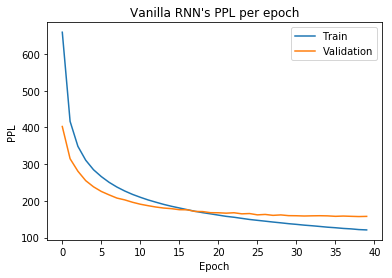
\includegraphics[scale=0.8]{Q4-1_RNN_epoch.png}
	\caption{Vanilla RNN's PPL per epoch}
	\label{fig:fig1}
\end{figure}

\begin{figure}[H]
	\centering
	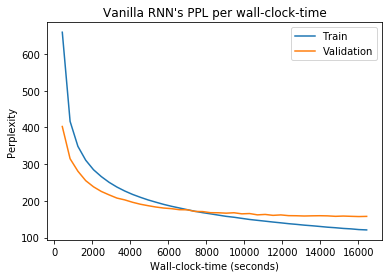
\includegraphics[scale=0.8]{Q4-1_RNN_clock.png}
	\caption{Vanilla RNN's PPL per wall-clock-time}
	\label{fig:fig2}
\end{figure}

\begin{figure}[H]
	\centering
	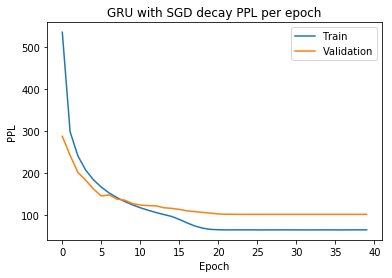
\includegraphics[scale=0.8]{Q4-1_GRU_SGDLR_epoch.png}
	\caption{GRU PPL per epoch}
	\label{fig:fig3}
\end{figure}

\begin{figure}[H]
	\centering
	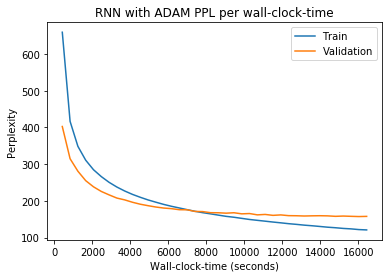
\includegraphics[scale=0.8]{Q4-1_RNN_ADAM_clock.png}
	\caption{GRU PPL per wall-clock-time}
	\label{fig:fig4}
\end{figure}

\begin{figure}[H]
	\centering
	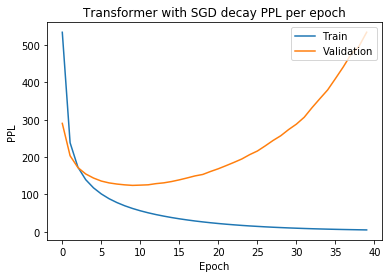
\includegraphics[scale=0.8]{Q4-1_TR_SGDLR_epoch.png}
	\caption{Transformer PPL per epoch}
	\label{fig:fig5}
\end{figure}

\begin{figure}[H]
	\centering
	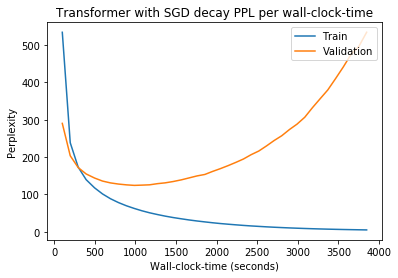
\includegraphics[scale=0.8]{Q4-1_TR_SGDLR_clock.png}
	\caption{Transformer PPL per wall-clock-time}
	\label{fig:fig6}
\end{figure}


\subsection{Exploration of optimizers}
In this section we will explore different optimizers for each of the previous models. Each model is run with two different optimizers with the hyperparameters as given in the assignment. 

\begin{itemize}
	\item[1)] \textbf{Results for Vanilla RNN:}
	The hyperparameters used for experiments 2 and 3 are given in the Table~\ref{table:3}.\\
	\begin{table}[H]
		\centering
		\begin{tabular}{||c c c c||} 
			\hline
			\textbf{Hyperparameters} & \textbf{Experiment 1} &\textbf{Experiment 2} & \textbf{Experiment 3}\\[0.5ex] 
			\hline
			Optimizer & ADAM & SGD & SGD\_LR\_SCHEDULE \\
			Learning rate & 0.0001 & 0.0001 & 1  \\
			Batch size &20 & 20 &20 \\
			Sequence length &35 & 35 & 35\\
			Hidden size & 1500 & 1500 & 512 \\
			Number of layers & 2 & 2 & 2 \\
			Dropout probability & 0.35 & 0.35 &0.35 \\[1ex]
			\hline
		\end{tabular}
		\caption{Vanilla RNN additionnal experiments' hyperparameters}
		\label{table:3}
	\end{table}
	%
	The results of these experiments are shown in  Table~\ref{table:3.1}. We notice that SGD performed worst and could not converge within 40 epochs, whereas ADAM performs best for the same number of epochs and the same hyperparameters. Additionnaly, the SGD\_LR\_SCHEDULE works better than SGD for a bigger learning rate and lower model capacity. In terms of training time, experiment 1 was the slowest, experiment 3 was the fastest while experiment 2 showed an average performance. 
	Given the above setting with the hyperparameters as shown in Table~\ref{table:3}, we conclude that the first experiment (ADAM) is best in terms of performance on the validation set. 
	\begin{table}[H]
		\centering
		\begin{tabular}{||c c c c||} 
			\hline
			\textbf{Result} & \textbf{Experiment 1} & \textbf{Experiment 2}& \textbf{Experiment 3} \\[0.5ex] 
			\hline
			Training PPL & 120.97 & 3008.63 & 229.56 \\
			Validation PPL & 157.82 & 2220.49 & 195.67  \\
			Average time processing per epoch (s) & 411 & 384 & 185 \\[1ex]
			\hline
		\end{tabular}
		\caption{Vanilla RNN results experiments}
		\label{table:3.1}
	\end{table}

\begin{figure}[H]
	\centering
	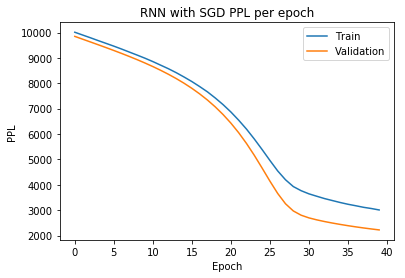
\includegraphics[scale=0.8]{Q4-2_RNN_SGD_epoch.png}
	\caption{Experiment 2 of RNN with SGD optimizer, learning curve by epoch}
	\label{fig:fig7}
\end{figure}

\begin{figure}[H]
	\centering
	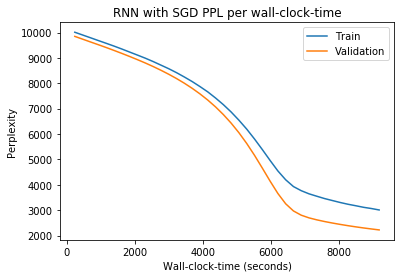
\includegraphics[scale=0.8]{Q4-2_RNN_SGD_clock.png}
	\caption{Experiment 2 of RNN with SGD optimizer, learning curve by time-clock}
	\label{fig:fig8}
\end{figure}

\begin{figure}[H]
	\centering
	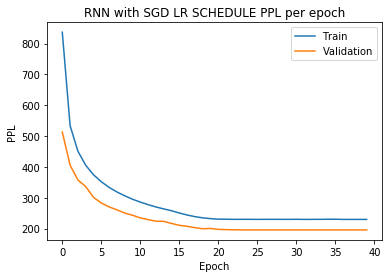
\includegraphics[scale=0.8]{Q4-2_RNN_SGD_LR_epoch.png}
	\caption{Experiment 3 of RNN with SGD decay optimizer, learning curve by epoch}
	\label{fig:fig9}
\end{figure}

\begin{figure}[H]
	\centering
	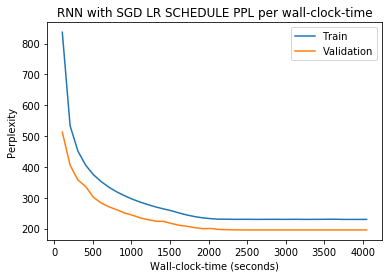
\includegraphics[scale=0.8]{Q4-2_RNN_SGD_LR_clock.png}
	\caption{Experiment 3 of RNN with SGD decay optimizer, learning curve by time-clock}
	\label{fig:fig10}
\end{figure}
	%
	\item[2)] \textbf{Results for GRU:}
	In the experiments 2 and 3, for GRU, we used the parameters given in Table~\ref{table:4}.\\
	%
	\begin{table}[H]
		\centering
		\begin{tabular}{||c c c c||} 
			\hline
			\textbf{Hyperparameters} &\textbf{Experiment 1} & \textbf{Experiment 2} & \textbf{Experiment 3}\\[0.5ex] 
			\hline
			Optimizer & SGD\_LR\_SCHEDULE & SGD & ADAM \\
			Learning rate & 10 & 10 & 0.0001   \\
			Batch size & 20 & 20 &20 \\
			Sequence length & 35 & 35 & 35\\
			Hidden size & 1500 & 1500 & 1500 \\
			Number of layers & 2 & 2 & 2 \\
			Dropout probability & 0.35 & 0.35 &0.35 \\[1ex]
			\hline
		\end{tabular}
		\caption{RNN with GRU additionnal experiments' hyperparameters}
		\label{table:4}
	\end{table}
	%
	The results are shown in Table~\ref{table:4.1}. We notice that SGD\_LR\_SCHEDULE performed best on the validation set, which indicates that it might also generalize well.  With a larger learning rate, SGD performed better than on the Vanilla RNN. ADAM's performance on the training set was best, but its variance was greater than SGD\_LR\_SCHEDULE, which may indicate that the model starts to overfit.
	\begin{table}[H]
		\centering
		\begin{tabular}{||c c c c||} 
			\hline
			\textbf{Result} & \textbf{Experiment 1} & \textbf{Experiment 2}& \textbf{Experiment 3} \\[0.5ex] 
			\hline
			Training PPL & 65.85& 50.33& 59.98 \\
			Validation PPL & 102.63 & 121.36 & 113.71  \\
			Average time processing per epoch (s) & 668 & 648 & 675 \\[1ex]
			\hline
		\end{tabular}
		\caption{First experiment results}
		\label{table:4.1}
	\end{table}

\begin{figure}[H]
	\centering
	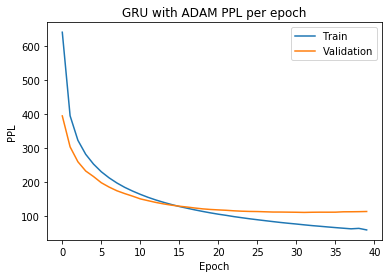
\includegraphics[scale=0.8]{Q4-2_GRU_ADAM_epoch.png}
	\caption{Experiment 2 of GRU with ADAM optimizer, learning curve by epoch}
	\label{fig:fig11}
\end{figure}

\begin{figure}[H]
	\centering
	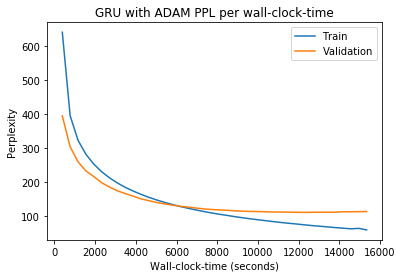
\includegraphics[scale=0.8]{Q4-2_GRU_ADAM_clock.png}
	\caption{Experiment 2 of GRU with ADAM optimizer, learning curve by time-clock}
	\label{fig:fig12}
\end{figure}

\begin{figure}[H]
	\centering
	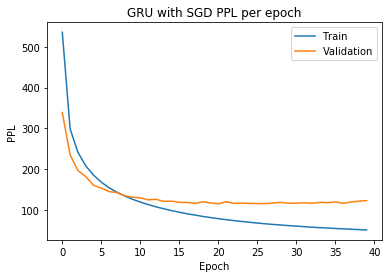
\includegraphics[scale=0.8]{Q4-2_GRU_SGD_epoch.png}
	\caption{Experiment 3 of GRU with SGD optimizer, learning curve by epoch}
	\label{fig:fig13}
\end{figure}

\begin{figure}[H]
	\centering
	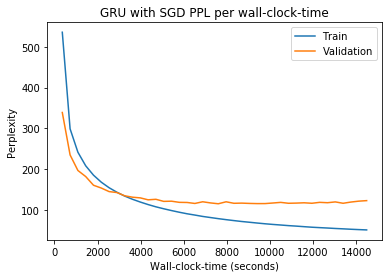
\includegraphics[scale=0.8]{Q4-2_GRU_SGD_clock.png}
	\caption{Experiment 3 of GRU with SGD optimizer, learning curve by time-clock}
	\label{fig:fig14}
\end{figure}
	%
		\item[3)] \textbf{Results for Transformer:}
		The following parameters were used:
		%
		\begin{table}[H]
			\centering
			\begin{tabular}{||c c c c||} 
				\hline
				\textbf{Hyperparameters} &\textbf{Experiment 1} & \textbf{Experiment 2} & \textbf{Experiment 3}\\[0.5ex] 
				\hline
				Optimizer & SGD\_LR\_SCHEDULE & SGD & ADAM\\
				Learning rate & 20 & 20 & 0.001  \\
				Batch size & 128 & 128 & 128 \\
				Sequence length & 35 & 35 & 35\\
				Hidden size & 512 & 512 & 512 \\
				Number of layers & 6 & 6 & 2 \\
				Dropout probability & 0.9 & 0.9 &0.9 \\[1ex]
				\hline
			\end{tabular}
			\caption{The hyperparameters for additional Transformer experiments}
			\label{table:5}
		\end{table}
The following are the results for the transformer:
\begin{table}[H]
	\centering
	\begin{tabular}{||c c c c||} 
		\hline
		\textbf{Result} & \textbf{Experiment 1} & \textbf{Experiment 2}& \textbf{Experiment 3} \\[0.5ex] 
		\hline
		Training PPL & 63.01 & 50.21 & 33.88  \\
		Validation PPL & 147.11 & 126.07  & 163.91  \\
		Average time processing per epoch (s) & 163  & 176  & 164 \\[1ex]
		\hline
	\end{tabular}
	\caption{First experiment results}
	\label{table:5.1}
\end{table}

\begin{figure}[H]
	\centering
	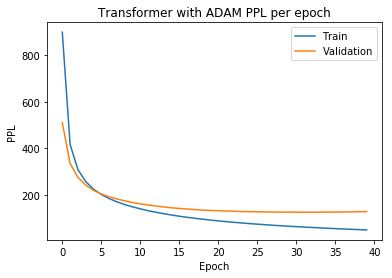
\includegraphics[scale=0.8]{Q4-2_TR_ADAM_epoch.png}
	\caption{Experiment 2 of Transformer with ADAM optimizer, learning curve by epoch}
	\label{fig:fig15}
\end{figure}

\begin{figure}[H]
	\centering
	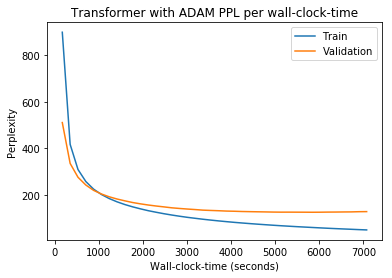
\includegraphics[scale=0.8]{Q4-2_TR_ADAM_clock.png}
	\caption{Experiment 2 of Transformer with ADAM optimizer, learning curve by time-clock}
	\label{fig:fig16}
\end{figure}

\begin{figure}[H]
	\centering
	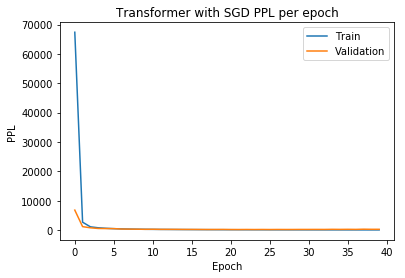
\includegraphics[scale=0.8]{Q4-2_TR_SGD_epoch.png}
	\caption{Experiment 3 of Transformer with ADAM optimizer, learning curve by epoch}
	\label{fig:fig17}
\end{figure}

\begin{figure}[H]
	\centering
	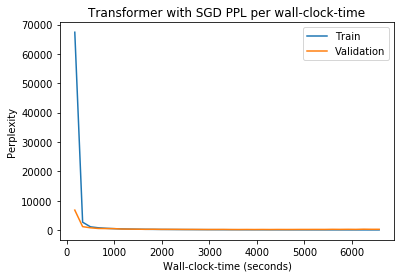
\includegraphics[scale=0.8]{Q4-2_TR_SGD_clock.png}
	\caption{Experiment 3 of Transformer with ADAM optimizer, learning curve by time-clock}
	\label{fig:fig18}
\end{figure}

\end{itemize}
%


%For the next experiment we will use the best optimizer so far. In order to improve its performance we will do a hyperparameter tuning.


\subsection{Exploration of hyperparmeters}

In this section we will present the result of the validation processus which consist on finding the best hyperparameters per architecture and per optimizer. This operation has required more than 30 experiments, from chich we will take the best 3 per architecture, which is 6 in total. The Figure~\ref{label} present the result of these experiments:

\begin{figure}[H]
	\centering
	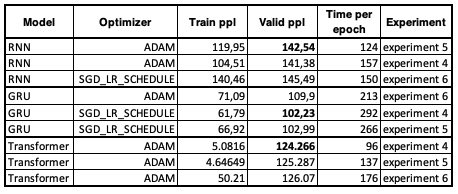
\includegraphics[scale=0.6]{Q4-3_Summury.png}
	\caption{Summury of the best experimentation of the 3 models}
	\label{fig:fig19}
\end{figure}

In the following table we will show all the hyperparameters values that we used for those experiments:

\begin{figure}[H]
	\centering
	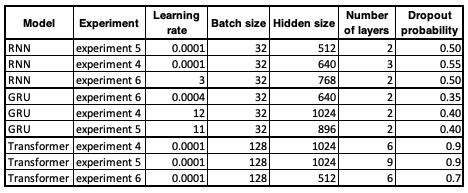
\includegraphics[scale=0.6]{Q4-3_Hyperparameters.png}
	\caption{Summury of the hyperparameters used in the experimentation above}
	\label{fig:fig19b}
\end{figure}


We will show next the learning curves of each experiment:
\begin{itemize}
	\item Vanilla RNN:
	\begin{figure}[H]
		\centering
		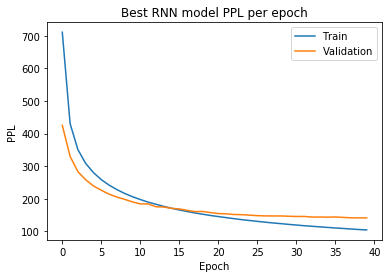
\includegraphics[scale=0.8]{Q4-3_RNN_1epoch.png}
		\caption{Experiment 4: Best result for RNN which gets better result than the baseline (learning curve by epoch)}
		\label{fig:fig20}
	\end{figure}
\begin{figure}[H]
	\centering
	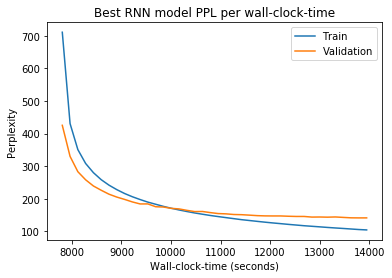
\includegraphics[scale=0.8]{Q4-3_RNN_1time.png}
	\caption{Experiment 4: Best result for RNN which gets better result than the baseline (learning curve by time-clock)}
	\label{fig:fig20b}
\end{figure}
	
	\begin{figure}[H]
		\centering
		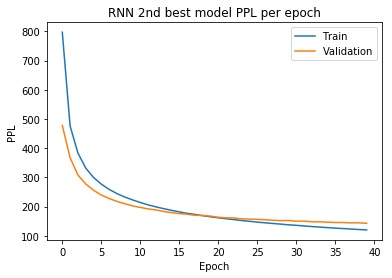
\includegraphics[scale=0.8]{Q4-3_RNN_2epoch.png}
		\caption{Experiment 5: 2nd best result for RNN (learning curve by epoch)}
		\label{fig:fig21}
	\end{figure}
\begin{figure}[H]
	\centering
	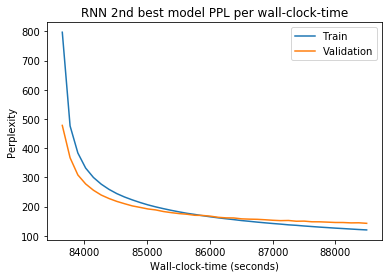
\includegraphics[scale=0.8]{Q4-3_RNN_2time.png}
	\caption{Experiment 5: 2nd best result for RNN (learning curve by time-clock)}
	\label{fig:fig21b}
\end{figure}
	
	\begin{figure}[H]
		\centering
		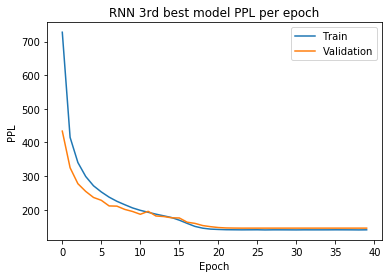
\includegraphics[scale=0.8]{Q4-3_RNN_3epoch.png}
		\caption{Experiment 6: 3rd best result for RNN (learning curves per epoch)}
		\label{fig:fig22}
	\end{figure}
\begin{figure}[H]
	\centering
	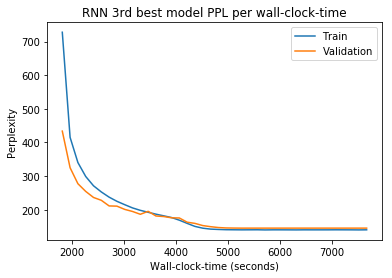
\includegraphics[scale=0.8]{Q4-3_RNN_3time.png}
	\caption{Experiment 6: 3rd best result for RNN (learning curves per clock)}
	\label{fig:fig22b}
\end{figure}


\item GRU:

\begin{figure}[H]
	\centering
	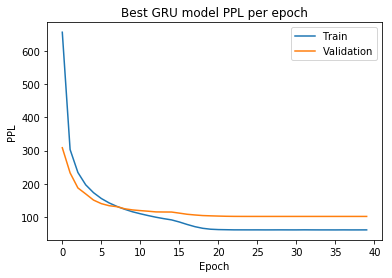
\includegraphics[scale=0.8]{Q4-3_GRU_1epoch.png}
	\caption{Experiment 4: Best result for GRU which gets better result than the baseline (learning curve by epoch)}
	\label{fig:fig20GRU}
\end{figure}
\begin{figure}[H]
	\centering
	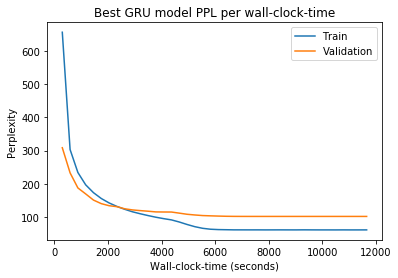
\includegraphics[scale=0.8]{Q4-3_GRU_1time.png}
	\caption{Experiment 4: Best result for GRU which gets better result than the baseline (learning curve by time-clock)}
	\label{fig:fig20bGRU}
\end{figure}

\begin{figure}[H]
	\centering
	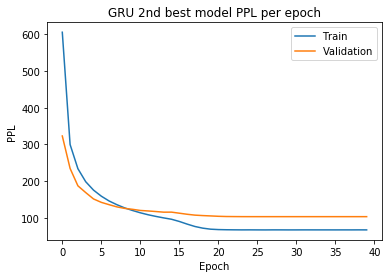
\includegraphics[scale=0.8]{Q4-3_GRU_2epoch.png}
	\caption{Experiment 5: 2nd best result for GRU (learning curve by epoch)}
	\label{fig:fig21GRU}
\end{figure}
\begin{figure}[H]
	\centering
	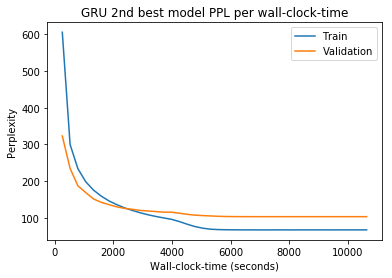
\includegraphics[scale=0.8]{Q4-3_GRU_2time.png}
	\caption{Experiment 5: 2nd best result for GRU (learning curve by time-clock)}
	\label{fig:fig21bGRU}
\end{figure}

\begin{figure}[H]
	\centering
	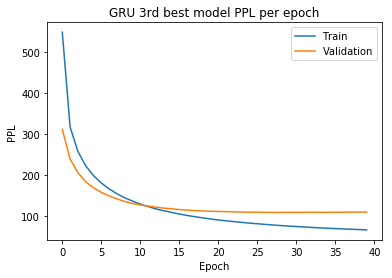
\includegraphics[scale=0.8]{Q4-3_GRU_3epoch.png}
	\caption{Experiment 6: 3rd best result for GRU (learning curves per epoch)}
	\label{fig:fig22GRU}
\end{figure}
\begin{figure}[H]
	\centering
	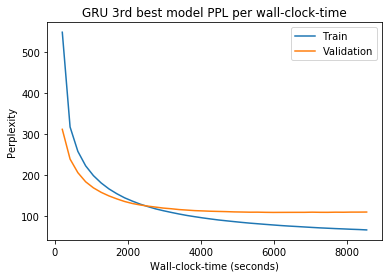
\includegraphics[scale=0.8]{Q4-3_GRU_3time.png}
	\caption{Experiment 6: 3rd best result for GRU (learning curves per clock)}
	\label{fig:fig22bGRU}
\end{figure}


\item Transformer:

\begin{figure}[H]
	\centering
	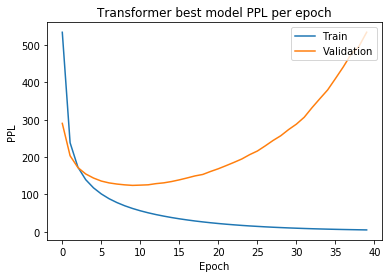
\includegraphics[scale=0.8]{Q4-3_TR_1epoch.png}
	\caption{Experiment 4: Best result for Transformer which gets better result than the baseline (learning curve by epoch)}
	\label{fig:fig20TR}
\end{figure}
\begin{figure}[H]
	\centering
	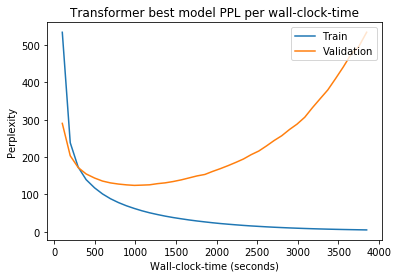
\includegraphics[scale=0.8]{Q4-3_TR_1time.png}
	\caption{Experiment 4: Best result for Transformer which gets better result than the baseline (learning curve by time-clock)}
	\label{fig:fig20bTR}
\end{figure}

\begin{figure}[H]
	\centering
	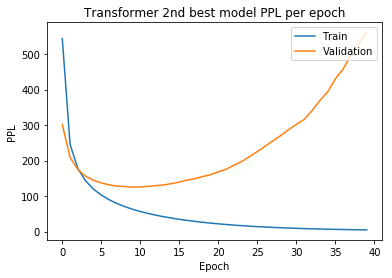
\includegraphics[scale=0.8]{Q4-3_TR_2epoch.png}
	\caption{Experiment 5: 2nd best result for Transformer (learning curve by epoch)}
	\label{fig:fig21TR}
\end{figure}
\begin{figure}[H]
	\centering
	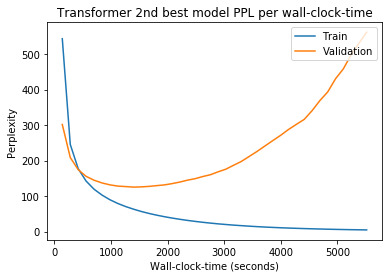
\includegraphics[scale=0.8]{Q4-3_TR_2time.png}
	\caption{Experiment 5: 2nd best result for Transformer (learning curve by time-clock)}
	\label{fig:fig21bTR}
\end{figure}

\begin{figure}[H]
	\centering
	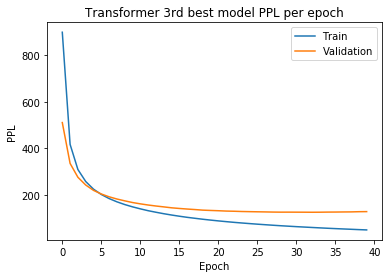
\includegraphics[scale=0.8]{Q4-3_TR_3epoch.png}
	\caption{Experiment 6: 3rd best result for Transformer (learning curves per epoch)}
	\label{fig:fig22TR}
\end{figure}
\begin{figure}[H]
	\centering
	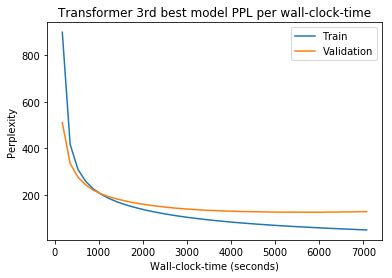
\includegraphics[scale=0.8]{Q4-3_TR_3time.png}
	\caption{Experiment 6: 3rd best result for Transformer (learning curves per clock)}
	\label{fig:fig22bTR}
\end{figure}

\end{itemize}


4. Make 2 plots for each optimizer; one which has all of the validation curves for that optimizer
over epochs and one over wall-clock-time.
5. Make 2 plots for each arcitecture; one which has all of the validation curves for that architecture
over epochs and one over wall-clock-time.

\subsection{Discussion}
\begin{enumerate}
	\item What did you expect to see in these experiments, and what actually happens? Why do you
think that happens?

We expected that the GRU will get better performance than the vanilla RNN, which was the case. In terms of time processing we have expected that GRU will be slower than the other architecture  which was the case eather given his number of calculations.

In other hand, we expected the Transformer will outperfom the other architectures in terms of perplexity on the validation set and in terms of time processing. It was the case for the time processing but, it wasn't the best model in all cases.

In terms of optimizer, we expected that ADAM will get better result, but SGD with learning rate decay was better optimizer.

\item Referring to the learning curves, qualitatively discuss the differences between the three optimizers
in terms of training time, generalization performance, which architecture they're best
for, relationship to other hyperparameters, etc.

Assuming that the comparison here was made with a set of hyperparameters that give a fair baseline for all the models, we can say that there is no universal best optimizer regardeless of the model architecture. In fact, each model architecture works better with a suited optimizer. Howerver, we notice that ADAM is a very powerfull optimizer that can make the model converge very quickly. However, if not well-tuned it could make the model overfit the training data. \\

3. Which hyperparameters+optimizer would you use if you were most concerned with wallclock
time? With generalization performance? In each case, what is the "cost" of the good
performance (e.g. does better wall-clock time to a decent loss mean worse nal loss? Does
better generalization performance mean longer training time?)

If we are more concerned with the time processing we would use Transformer which is clearly very fast than the other architecture. And the cost of good performance for this kind of architecture is to have a lot of data and a very good tuning using regularization.
If we are more concerned with generalization, we would use GRU as it seems to be less sensitive to overfitting better than Transformer as shown in Figure~\ref{fig:fig20TR}. In this case, the cost of a good performance is the time processing as GRU takes more time train and it is hard to get good hyperparamers.

Training a model for a long time does not mean better performance, because the model will be either in a stationary regime or strat overfitting

4. Which architecture is most "reliable" (decent generalization performance for most hyperparameter+
optimizer settings), and which is more unstable across settings?
I would use GRU because it is a more robust architecture and it gets the better result. Transformer is a fancy architecture but it was the only architecture that was unstable during the experiments

5. Describe a question you are curious about and what experiment(s) (i.e. what architecture/
optimizer/hyperparameters) you would run to investigate that question.



\end{enumerate}